\chapter{Choix technologiques}
    Le choix des technologies utilisées pour le développement du logiciel a été le point d'entrée du projet. Les enjeux sont cruciaux, car la vitesse du développement et la productivité des développeurs dépend du choix des outils qui sont soit déjà connus, soit à apprendre. Le tout a donc été de trouver un accord au sein du binôme sur les technologies à employer. Cette étape de brainstorming a duré environ deux heures.

    \section{Language C++}
        La première étape dans cette reflexion a été de choisir le language dans lequel il serait développé: la contrainte qui nous était imposée 
        était le choix entre le language C et ses dérivés.
        \\ Le C est un language de programmation généraliste et bas niveau\footnote{Près de la machine. En C beaucoup de résponsabilités sont laissées au développeur, comme l'allocation mémoire} inventé dans les années 1970. C'est un des language les plus utilisés au monde, pionnier du monde informatique, qui a inspiré nombre d'autres languages et donné naissance à des dérivés comme le C\#\footnote{Prononcer ``C sharp''}, 
        l'Objective-C ou encore le C++.
        \\ Notre choix s'est porté sur ce dernier, car il intègre bon nombre de concepts plus récents en programmation comme la POO\footnote{Programmation
        orientée objet} qui nous sont familiers. Il n'est également d'aucune affiliation particulière avec les entreprises: le C\# étant développé par microsoft
        et l'objective-C par Apple.
        \\ Une fois le language choisi, nous nous sommes intéressés aux différents frameworks\footnote{Espace de travail - sorte de grande bibliothèque 
        de programmation}
        graphiques disponibles.

    \section{Framework Qt}
        \begin{figure}[h]
            \begin{center}
                
\includegraphics[scale=0.25]{Qt.png}
            \end{center}

            \caption{Logo de Qt}
            \label{Qt}
        \end{figure}

        La motivation derrière l'utilisation de Qt résulte tout d'abord de la volonté d'avoir un programme multi-plateforme. Le développement du programme étant fait dans un environnement linux, et avec une majorité d'ordinateurs tournant sous windows, la nécessité d'avoir un programme portatif était évidente.
        \\ Un rapide tour d'horizon sur les différents frameworks/libraries multi-plateformes montre qu'il n'y a essentiellement que trois grand projet: WxWidgets, GTK et Qt.

    \newpage
        
        L'avantage de Qt par rapport à ses concurrents est qu'il jouit d'une très large communauté, et est maintenu par Nokia. C'est un framework très moderne allant jusqu'à étendre le C++ pour lui apporter des fonctionnalités non natives. Il permet donc le développement dans un environnement plus haut niveau, au détriment des performances du programme, que nous avons jugées négligeables étant donnée l'échelle du programme.
        \\ Enfin, en plus de faciliter le développement du coeur du programme, Qt à l'avantage de proposer un IDE\footnote{Integrated development environment}, Qt Creator, qui dispose d'une auto-complétion très poussée ainsi qu'un éditeur WYSIWYG\footnote{What you see is what you get - il n'y a qu'à dessiner pour obtenir ce que l'ont veux} d'interface graphique.

        \begin{figure}[h]
            \begin{center}
                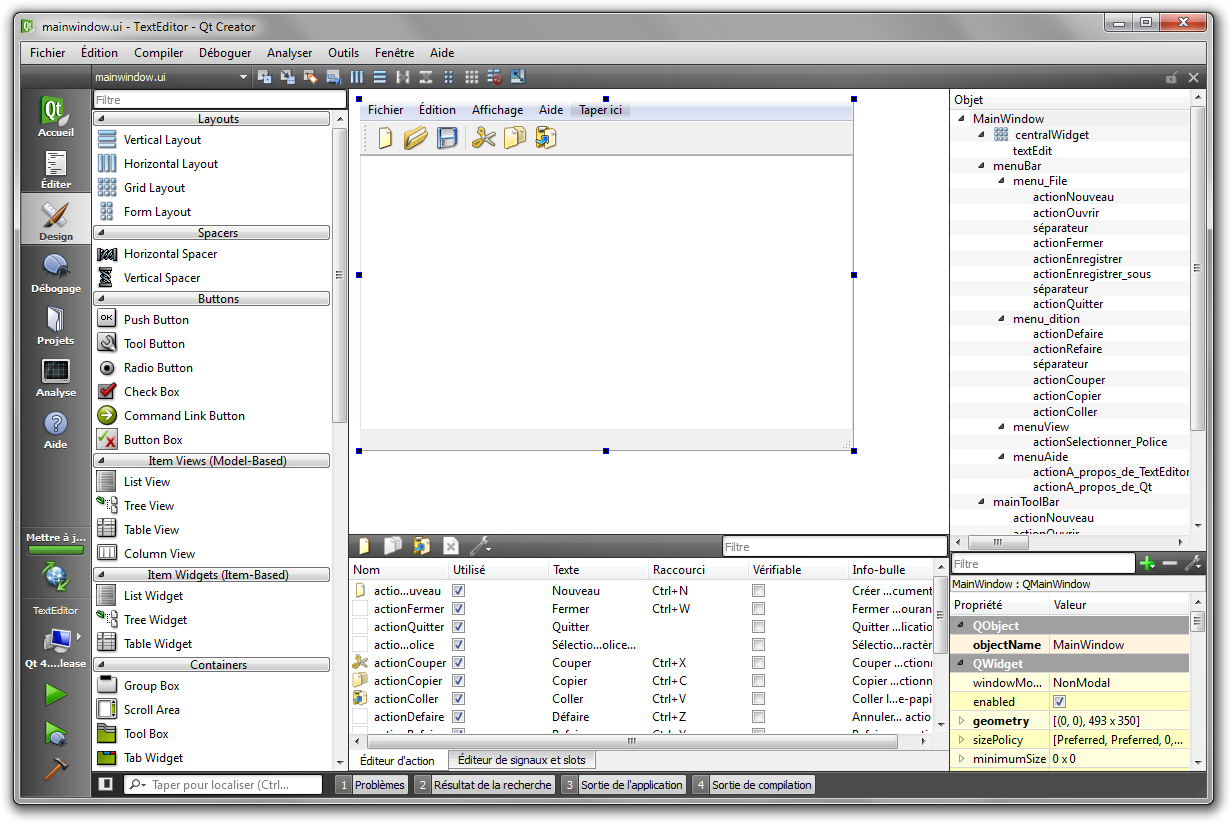
\includegraphics[scale=0.3]{Qt_creator.png}
            \end{center}

            \caption{Éditeur d'interface WYSIWYG de Qt Creator}
            \label{Qt Creator}
        \end{figure}

        L'utilisation de l'éditeur graphique de Qt Creator a fait gagner beaucoup de temps sur le développement. Malgré sa puissance et sa simplicité d'utilisation, il n'en reste pas moins limité: seul un certain nombre de widget prédéfinis peuvent être utilisés. L'utilisation de widgets plus complexes ont été requis pour la réalisation de la liste des variables, ils ont donc été développés main (Voir \ref{detailedlist.hpp} detailedlist.hpp).

    \newpage

    \section{Gestionnaire de version et travail collaboratif Git}
        \paragraph{}
            Bien que n'étant qu'en binôme, travailler en équipe sur un même code sans outil approprié se révèle souvent être un enfer. En effet, la modification d'un fichier peut entrainer des incompatibilités et des bugs dans le reste du programme. Et c'est à ce genre de problèmes que vient répondre un gestionnaire de version.
            \\ Tout comme les frameworks graphiques, il existe plusieurs solutions sur le marché, on retiendra essentiellement svn et git. Le choix de git fût immédiat car maîtrisé par l'ensemble de l'équipe. 

        \paragraph{}
            Git a été créé en 2005 par Linus Torvalds, créateur de noyau linux, devant la nécessité de canaliser et organiser les contributions des milliers de contributeurs de linux. C'est le gestionnaire de version le plus utilisé, et est un réel standard dans le monde du développement logiciel.

        \begin{figure}[h]
            \begin{center}
                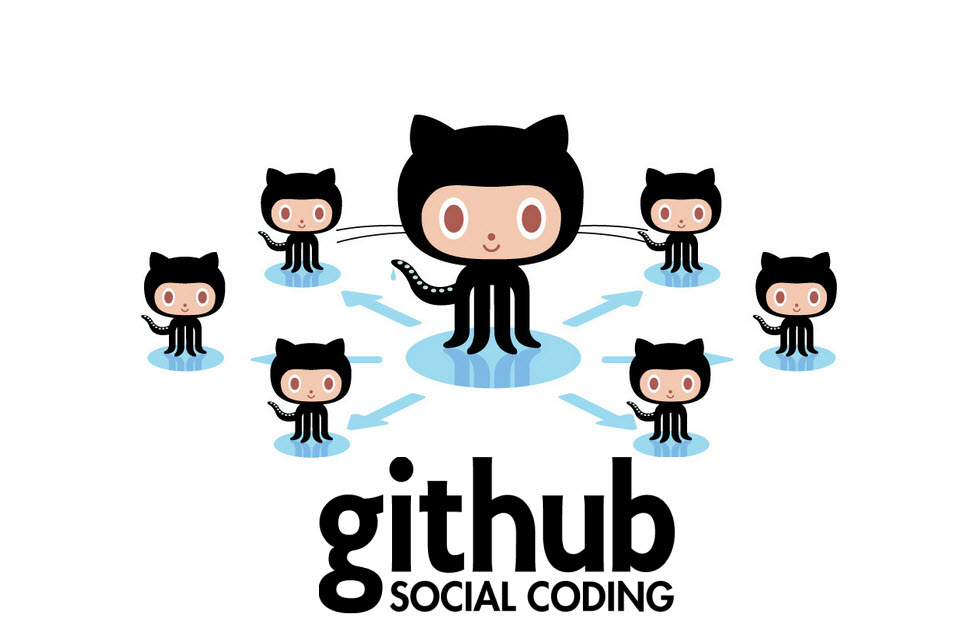
\includegraphics[scale=0.3]{logo_github.jpg}
            \end{center}

            \caption{Logo de github}
            \label{github}
        \end{figure}

        \paragraph{}
            Git est un outil déscentralisé, un service : il doit être herbergé par un serveur. Là ou il est possible d'être indépendant et d'héberger son propre serveur github, nous avons préferé nous rabattre sur un hébergeur gratuit et public, github.
            \\ Ce choix est motivé et par la facilité d'utilisation qu'offre github, mais aussi par la volonté d'avoir un programme libre. Github met ainsi à 
            disposition librement et pour tous notre programme, sous la licence de notre choix\footnote{Ici MIT}.
            


    \newpage

    \section{Générateur de documentation Doxygen}
        \paragraph{}
            Doxygen est un générateur de documentation à partir du code source. Un des problèmes lié au travail de groupe et auquel git ne répond pas, est la maintanibilité et la lisibilité du code, et c'est là que doxygen apporte des solutions.
            \\ Avec une syntaxe claire et rigoureuse de commentaires judicieusement placés sur chaque fonction et instruction utile, le code produit par une personne devient limpide pour une autre personne formée à utiliser doxygen. De plus, la documentation générée (sous format html, pdf..) permet d'avoir une vue d'ensemble sur le code, notamment grâce à des graphiques représentant les interactions entre les classes.

        \begin{lstlisting}[frame=single, language=C++, caption=Exemple de  commentaire utilisant la syntaxe de doxygen] 
/**
 * @brief generate a Node tree representation of a tokenList
 *
 * @param tokens the tokenList to parse
 * @return a Node tree representation of the tokenlist
 */

Node* generateTree(QList<Token> tokens)
        \end{lstlisting}


        \paragraph{}
            Le dernier avantage, et pas des moindres, est que pour tout nouveau contributeur dans le projet, l'apprentissage de la structure du logiciel est bien plus rapide que sans documentation. Le choix ayant été fait d'avoir un programme libre, il a semblé naturel de fournir une documentation allant avec le programme.
            
        \paragraph{}
            Un autre choix ayant été fait au niveau des commentaires a été de les rédiger entièrement en Anglais. Dans le monde de l'informatique, l'anglais est omniprésent: au niveau des documentations, des forums, des ressources. Commenter en français implique que la portabilité du programme ne pourra se faire qu'en millieux francophone et qu'aucune contribution ne pourra être apportée par quelqu'un ne maîtrisant pas le français. De l'autre côté, l'anglais est compris pratiquement universellement. 
        
